
\documentclass{beamer}

\usepackage{algpseudocode, color, colortbl, listings, MnSymbol}

\usepackage{hyperref}
\hypersetup{
    colorlinks=true,
    urlcolor=blue,
}

\usetheme{Montpellier}
\usecolortheme{rose}

% page numbers, from
% https://tex.stackexchange.com/questions/137022/how-to-insert-page-number-in-beamer-navigation-symbols
\expandafter\def\expandafter\insertshorttitle\expandafter{%
  \insertshorttitle\hfill%
  \insertframenumber\,/\,\inserttotalframenumber}

\definecolor{Gray}{gray}{0.8}
\newcolumntype{g}{>{\columncolor{Gray}}c}

\newcommand{\stanza}{ \\~\ }

\title{20. Longest Common Subsequence}
\subtitle{CPSC 535}
\author{Kevin A. Wortman}
\institute{ 
\includegraphics[height=2cm]{csuf-logo-cmyk} }
\date{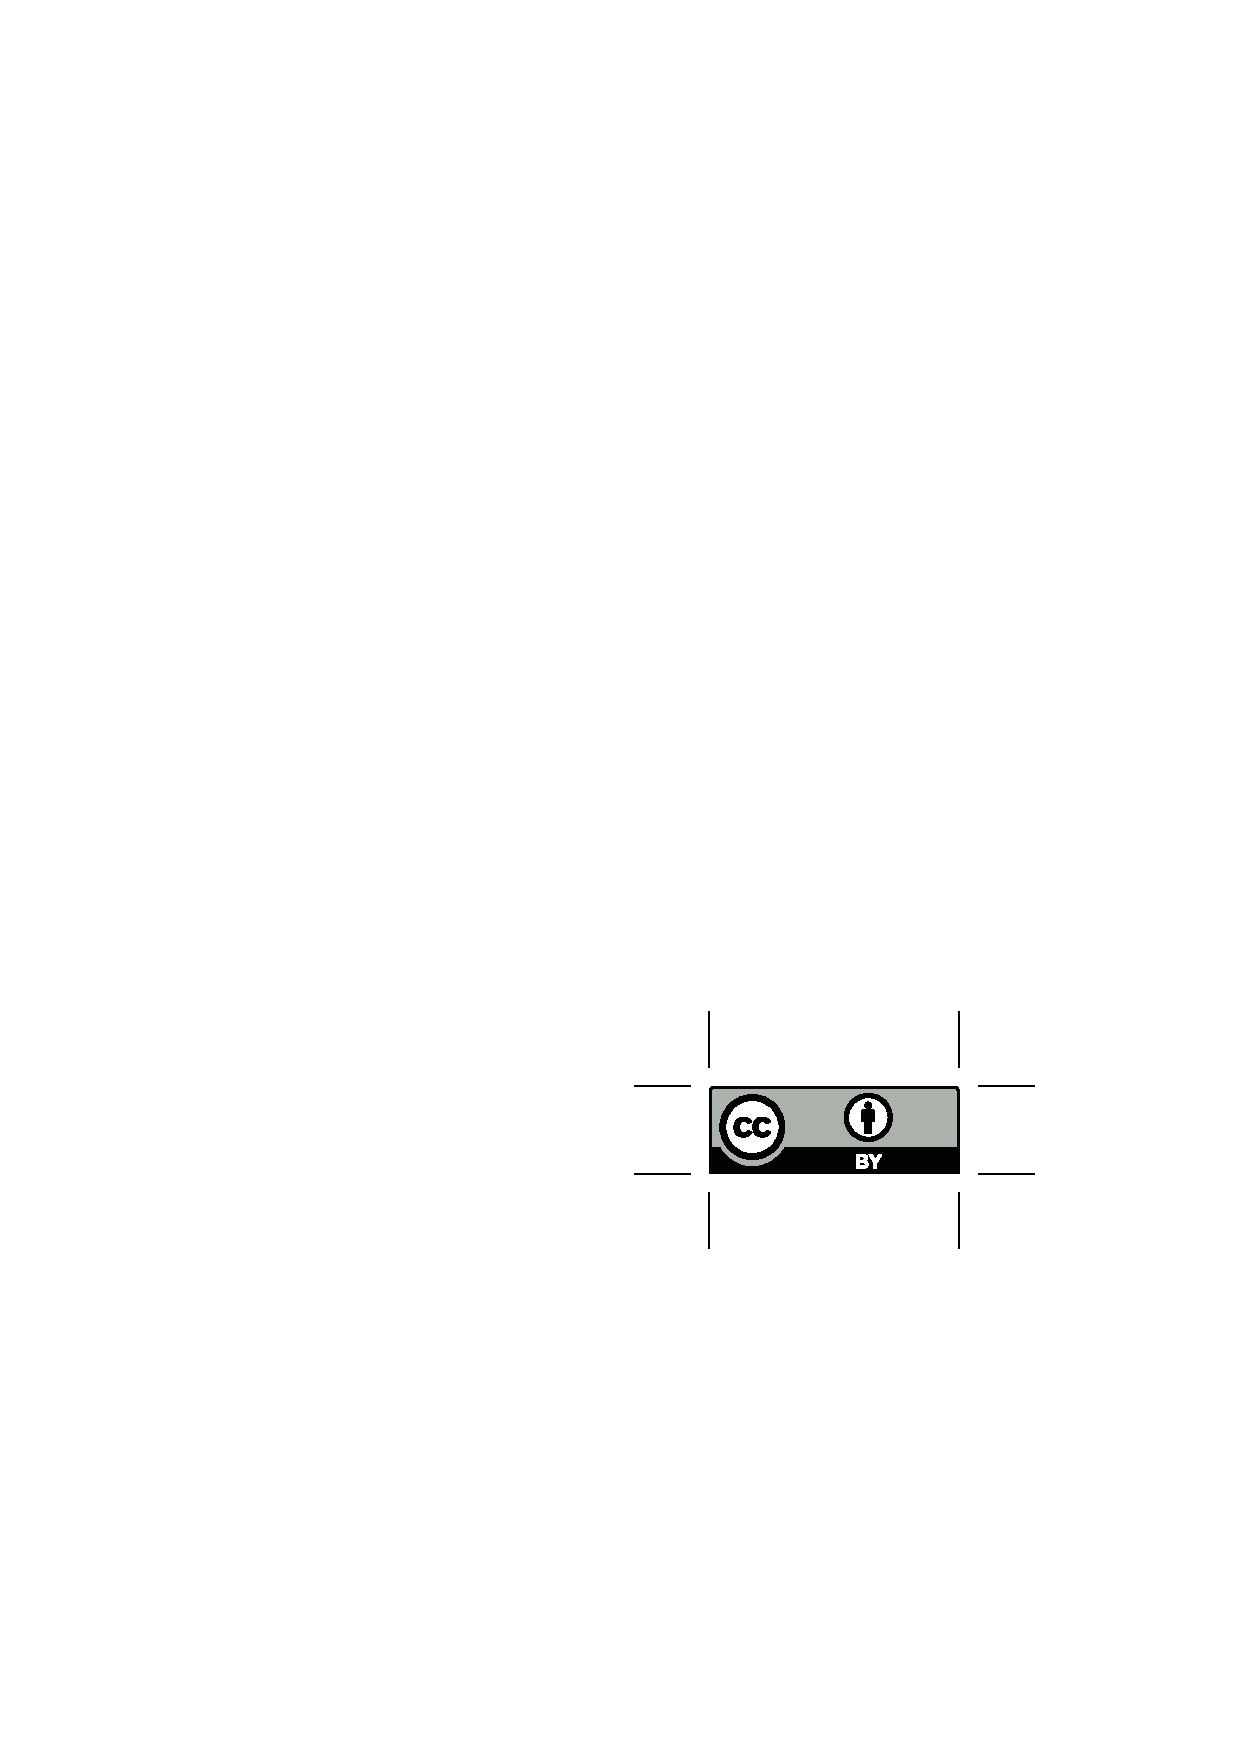
\includegraphics[height=14pt]{by} \\

{\tiny
This work is licensed under a
\href{http://creativecommons.org/licenses/by/4.0/}{Creative Commons Attribution 4.0 International License}.
}}

\begin{document}

\begin{frame}
  \titlepage
\end{frame}

\begin{frame} \frametitle{1D vs 2D Dynamic Programming}
  \begin{itemize}
  \item Previous class: rod cutting
    \begin{itemize}
    \item Recursive solution:
      $r_n = \max_{1 \leq i \leq n} (p_i + r_{n-i}) $
    \item References a 1D sequence $r_j:$
      $r_n = \ldots r_{n-i} \ldots$
    \item $\therefore$ initializing $r[j]$ involves one non-nested loop; $\Theta(n)$
    \item Call this \textbf{1D dynamic programming}
    \end{itemize}
  \item Now: longest common subsequence (LCS)
    \begin{itemize}
    \item Recursive solution: $c[i][j] = \ldots c[i-1,j-1]+1 \ldots c[i,j-1] \ldots c[i-1,j] \ldots$
    \item References a 2D matrix $c[i][j]$
    \item $\therefore$ initializing $c[i][j]$ involves two nested loops; $\Theta(n^2)$
    \item Call this \textbf{2D dynamic programming}
    \end{itemize}
  \end{itemize}
\end{frame}

\begin{frame} \frametitle{Subsequences}
  \begin{itemize}
  \item Let $X=\langle x_1, x_2, \ldots, x_m \rangle$ and $Y=\langle y_1, y_2, \ldots, y_n \rangle$ be two sequences
  \item Define \textbf{prefix} notation: $X_k = \langle x_1, \ldots, x_k \rangle; X_0 = \langle \rangle$
  \item Informally: a \textbf{subsequence} of $Y$ is a copy of $Y$ with some elements removed
  \item Formally: $X$ is a \textbf{subsequence} of $Y$ if there exists an increasing sequence of indices $\langle i_1, i_2, \ldots, i_k \rangle$ such that, for all $j \in [1, k], x_j = y_{i_j}$
  \item Example: for $X=\langle B, C, D, B\rangle$ and $Y=\langle A, B, C, B, D, A, B \rangle,$ $X$ is a subsequence of $Y$ with index sequence $\langle 2, 3, 5, 7 \rangle$
  \end{itemize}
\end{frame}

\begin{frame} \frametitle{Common Subsequence}
  \begin{itemize}
  \item $Z$ is a \textbf{common subsequence} of $X$ and $Y$ if $Z$ is a subsequence of both $X$ and $Y$
  \item a \textbf{longest common subsequence} is a common subsequence of maximum length
  \item Example: let $X=\langle A, B, C, B, D, A, B \rangle $ (same) and $Y=\langle B, D, C, A, B, A \rangle$ (different)
  \item $Z=\langle B, C, A \rangle$ is a common subsequence
  \item $Z=\langle B, C, B, A \rangle$ is a longest common subsequence
  \end{itemize}
\end{frame}

\begin{frame} \frametitle{Longest Common Subsequence}

  \emph{Longest Common Subsequence (LCS) value problem} \\
  \textbf{input:} sequences $X=\langle x_1, x_2, \ldots, x_m \rangle$ and $Y=\langle y_1, y_2, \ldots, y_n \rangle$
  \textbf{output:} the length of a longest common subsequence of $X$ and $Y$ \stanza

  \emph{Longest Common Subsequence (LCS) solution problem} \\
  \textbf{input:} (same) \\
  \textbf{output:} a longest common subsequence of $X$ and $Y$ \stanza
  
\end{frame}

\begin{frame} \frametitle{Step 1: Characterize a baseline solution}
  \begin{itemize}
  \item \textbf{Idea:} brute force
  \item Enumerate every subsequence $Z$ of $X$; check if each $Z$ is also a subsequence of $Y$; keep the maximum-length acceptable $Z$
  \item $\Theta((m+n)2^m)$ time
  \item Exponential; too slow
  \end{itemize}
\end{frame}    

\begin{frame} \frametitle{Step 1: Characterize a a solution recursively}
  \begin{itemize}
  \item Recall input: $X=\langle x_1, x_2, \ldots, x_m \rangle$ and $Y=\langle y_1, y_2, \ldots, y_n \rangle$
  \item Recall \emph{prefix:} $X_i$ is first $i$ elements of $X$
  \item We want to compute sequence $LCS(X, Y)$; need to define this recursively
  \item \textbf{Idea:} If last symbols $x_m=y_n$ match, then extend a shorter common subsequence:
    $LCS(X, Y) = LCS(X_{m-1}, Y_{n-1}) + \langle x_m \rangle$
  \item Else ($x_m \ne y_n$), have to omit $x_m$ or $y_n$ (or both)
    \begin{itemize}
    \item Omit $x_m$ (or both): $LCS(X, Y) = LCS(X_{m-1}, Y)$
    \item Omit $y_n$ (or both): $LCS(X, Y) = LCS(X, Y_{n-1})$
    \item Want \textbf{longest} so $LCS(X, Y) = \text{ longer of } LCS(X_{m-1}, Y) \text{ and } LCS(X, Y_{n-1})$
    \end{itemize}
  \end{itemize}
\end{frame}

\begin{frame} \frametitle{Example}
  \begin{itemize}
  \item Suppose $X=\langle A, B, A, D \rangle$ and $Y = \langle B, B, A, C, D \rangle$
  \item Last symbols match,  $x_4=y_5=D,$ so
    \begin{align*}
      LCS(X,Y) &= LCS(X_{m-1}, Y_{n-1}) \\
      &= LCS(\langle A, B, A \rangle, \langle B, B, A, C \rangle) + \langle D \rangle
    \end{align*}
  \item Now suppose $X=\langle A, B, A, C \rangle$ and $Y$ is the same
  \item Last symbols differ, $x_4=C$ but $y_5=D,$ so
    \begin{align*}
      LCS(X, Y) &= \text{ longer of } LCS(X_{m-1}, Y) \text{ and } LCS(X, Y_{n-1}) \\
      &= \text{longer of } LCS(\langle A, B, A \rangle, Y) \text{ and } LCS(X, \langle B, B, A, C \rangle)
    \end{align*}
  \end{itemize}
  
\end{frame}

\begin{frame} \frametitle{Step 2: Recursive solution}
  \begin{algorithmic}[1]
    \Function{LCS-LENGTH}{$X[0..m], Y[0..n]$}
    \If{ $m==0$ or $n==0$ }
      \State \Return 0
    \EndIf
    \If{ $x_m == y_n$ }
    \State \Return $LCS-LENGTH(X[0..m-1], Y[0..n-1]) + 1$
    \EndIf
    \State $a = LCS-LENGTH(X[0..m-1], Y)$
    \State $b = LCS-LENGTH(X, Y[0..n-1])$
    \State \Return $\max(a, b)$
    \EndFunction
  \end{algorithmic}  
\end{frame}

\begin{frame} \frametitle{Step 2: Recursive table definition}
  \begin{itemize}
  \item (Switching to \textbf{value} problem --- find length not subsequence)
  \item Create table (2D array) $c[i][j]$ with invariant
    \[ c[i][j] = \text{length of a LCS of } X_i \text{ and } Y_j \]
  \item Base cases: if $i=0$ or $j=0$, $c[i][j]=0$
  \item General cases:
    \begin{itemize}
    \item if $x_i=y_j$: $c[i][j] = c[i-1][j-1]+1$
    \item else, $c[i][j] = \max(c[i][j-1], c[i-1][j])$
    \end{itemize}
  \end{itemize}
\end{frame}

\begin{frame} \frametitle{Step 3: Pseudocode for \textbf{Bottom-Up} Dyn. Prog. Alg.}
  \begin{algorithmic}[1]
    \Function{LCS-LENGTH}{$X[0..m], Y[0..n]$}
    \State Create new 2D array $c[0..m][0..n]$
    \State \textbf{for} $i=0$ to $m:$ $c[i][0] = 0$
    \State \textbf{for} $j=1$ to $n:$ $c[0][j] = 0$
    \For { $i = 1 $ to $m$ }
      \For { $j = 1 $ to $n$ }
        \If{ $x_i == y_j$ }
          \State $c[i][j] = c[i-1][j-1]+1$
        \Else
          \State $c[i][j] = \max(c[i][j-1], c[i-1][j])$
        \EndIf
      \EndFor  
    \EndFor
    \State \Return $c[m][n]$
    \EndFunction
  \end{algorithmic}
\end{frame}

\begin{frame} \frametitle{Analysis}
  \begin{itemize}
  \item 2D array $c: \Theta(mn)$ space
  \item Base cases $j=0: \Theta(m)$ time
  \item Base cases $i=0: \Theta(n)$ time
  \item General cases: $\Theta(mn)$ time
  \item Total: $\Theta(m+n+mn)=\Theta(mn)$ time
  \item \textbf{Huge speedup:} $\Theta((m+n) 2^m) \longrightarrow \Theta(mn)$
  \item Exponential $\longrightarrow$ polynomial
  \end{itemize}
\end{frame}

\begin{frame} \frametitle{Improving Space Complexity}
  \begin{itemize}
  \item \textbf{Observe:} in the general-case loop, the only row indices used are $i$ and $i-1$
    \begin{itemize}
    \item Either $c[i][j] = c[i-1][j-1]+1$
    \item Or $c[i][j] = \max(c[i][j-1], c[i-1][j])$
    \end{itemize}
  \item $\therefore$ we only need two rows at a time
    \begin{itemize}
    \item 1) the current row $i$ we are initializing
    \item 2) the previous row $i-1$
    \end{itemize}
  \item Keep a \textbf{window} of only two rows
  \item This idea applies to many dynamic programming algorithms
  \end{itemize}
\end{frame}

\begin{frame} \frametitle{Space-Efficient Bottom-Up LCS}
  {\small
  \begin{algorithmic}[1]
    \Function{LCS-LENGTH}{$X[0..m], Y[0..n]$}
    \State Create arrays $prev[0..n]$ and $now[0..n]$, both filled with zeroes
    \For { $i = 1 $ to $m$ }
      \State swap($prev, now$)  
      \For { $j = 1 $ to $n$ }
        \If{ $x_i == y_j$ }
          \State $now[j] = prev[j-1]+1$
        \Else
          \State $now[j] = \max(now[j-1], prev[j])$
        \EndIf
      \EndFor
      \EndFor
    \State \Return $now[n]$
    \EndFunction
  \end{algorithmic}
  }
\end{frame}

\begin{frame} \frametitle{Space-Efficient Analysis}
  \begin{itemize}
  \item Space:
    \begin{itemize}
    \item Each array is $\Theta(n)$ space
    \item Total $\Theta(n)$ space
    \item (Better than $\Theta(mn)$)
    \end{itemize}
  \item Time:
    \begin{itemize}
    \item Initialize arrays: $\Theta(n)$
    \item General case loops: $\Theta(mn)$ time
    \item Total $\Theta(mn)$ time
    \item (Same as previous version)
    \end{itemize}
  \end{itemize}
\end{frame}

\end{document}
